\section{Grundlagen zu Wurzelsystemen}
\label{sec:grundlagen}

Dieser Abschnitt beinhaltet die für diese Arbeit benötigten Grundlagen zu Wurzelsystemen.  
Im Folgenden bezeichne $E$ stets einen \emph{\euklid ischen} Vektorraum, also einen $\R$\hyp{}Vektorraum mit Skalarprodukt $(\cdot,\cdot)$.

Einer \emph{Spiegelung} $\sigma$ ist eine orthogonale Abbildung auf $E$, welche eine \emph{Hyperebene}, also einen Unterraum der Kodimension $1$, punktweise fixiert und jeden Vektor des orthogonalen Komplements der Hyperebene auf sein Negatives abbildet.
Jeder Vektor $\alpha \in E \setminus \{0\}$ induziert eine \emph{Spiegelung} $\sigma_\alpha$ an der Hyperebene 
\begin{displaymath}
  P_\alpha := \spn(\{\alpha\})^\perp = \{\beta \in E \mid (\beta, \alpha) = 0\}.
\end{displaymath}
Definiert man nun $\langle \beta, \alpha \rangle := \tfrac{2 (\beta, \alpha)}{(\alpha, \alpha)}$, so gilt
\begin{displaymath}
  \label{eq:RF}
  \sigma_\alpha(\beta) 
  = \beta - \frac{2 (\beta, \alpha)}{(\alpha,\alpha)} \alpha 
  = \beta - \langle \beta, \alpha \rangle \alpha,\tag{RF}
\end{displaymath}
denn es gelten $\sigma_\alpha(\alpha) = -\alpha$ und $\sigma_\alpha(\beta) = \beta$ für alle $\beta \in P_\alpha$.
Man beachte, dass, im Gegensatz zum Skalarprodukt, der Ausdruck $\langle \beta, \alpha \rangle$ nur in der ersten Variablen linear ist.
Es gilt jedoch $\sign \langle \alpha, \beta \rangle = \sign (\alpha, \beta)$ für alle $\alpha, \beta \in E$.

\begin{lem}
  \label{lem:orthogonalRoots}
  %Es sei $E$ ein \textsc{euklid}ischer Vektorraum.
  Falls $(\alpha, \beta) = 0$ für $\alpha, \beta \in E$ gilt, so kommutieren die korrespondierenden Spiegelungen $\sigma_\alpha$ und $\sigma_\beta$.
\end{lem}

\begin{proof}
  Für $\gamma \in E$ gilt $\sigma_\alpha(\gamma) = \gamma - \langle \gamma, \alpha \rangle \alpha$. Da aus $(\alpha, \beta) = 0$ sofort $\langle \alpha, \beta \rangle = 0$ folgt, gilt also auch
  \begin{align*}
    \sigma_\beta \sigma_\alpha(\gamma) 
    &= \sigma_\alpha(\gamma) - \langle \sigma_\alpha(\gamma), \beta \rangle \beta \\
    &= \gamma - \langle \gamma, \alpha \rangle \alpha 
              - \langle \gamma- \langle \gamma, \alpha\rangle \alpha, \beta \rangle \beta \\
    &= \gamma - \langle \gamma, \alpha \rangle \alpha 
              - \langle \gamma, \beta \rangle \beta - \langle \gamma, \alpha \rangle \langle \alpha, \beta \rangle \beta \\
    &= \gamma - \langle \gamma, \alpha \rangle \alpha - \langle \gamma, \beta \rangle \beta.
  \end{align*} 
  Da dieser Ausdruck symmetrisch in $\alpha$ und $\beta$ ist, folgt $\sigma_\beta \sigma_\alpha = \sigma_\alpha \sigma_\beta$.
\end{proof}

Wir definieren nun das für diese Arbeit zentrale mathematische Objekt.

\begin{defn}
  Ein \emph{Wurzelsystem} $(E,\Phi)$ ist ein endlichdimensionaler \euklid ischer Vektorraum mit Skalarprodukt $(\cdot,\cdot)$ zusammen mit einer Teilmenge $\Phi \subseteq E$, welche die folgenden Eigenschaften besitzt:
  \begin{enumerate}[(R1)]
    \item\label{it:R1} Die Menge $\Phi$ ist endlich, sie erzeugt den Vektorraum $E$ auf und sie enthält nicht die $0$.
    \item\label{it:R2} Für alle $\alpha \in \Phi$ sind $\pm \alpha$ die einzigen Vielfachen von $\alpha$ in $\Phi$.
    \item\label{it:R3} Für alle $\alpha \in \Phi$ ist die Menge $\Phi$ invariant unter der Spiegelung $\sigma_\alpha$.
    \item\label{it:R4} Für alle $\alpha, \beta \in \Phi$ gilt $\langle \alpha, \beta \rangle \in \Z$.
  \end{enumerate}
  Spielt der Vektorraum $E$ nur eine untergeordnete Rolle, so bezeichnet man auch schlicht $\Phi$ als Wurzelsystem über $E$.
\end{defn}

\begin{bem}
  \begin{enumerate}
    \item In der Theorie symmetrischer Räume treten Systeme auf, die die Eigenschaften \hyperref[it:R1]{(R1)}, \hyperref[it:R3]{(R3)} und \hyperref[it:R4]{(R4)} aber nicht \hyperref[it:R2]{(R2)} erfüllen. 
      Diese Systeme werden auch als \emph{nichtreduzierte} Wurzelsysteme bezeichnet.
    \item In der Theorie der \textsc{coxeter}\hyp{}Gruppen treten Systeme auf, die die Eigenschaften \hyperref[it:R1]{(R1)}, \hyperref[it:R2]{(R2)} und \hyperref[it:R3]{(R3)} aber nicht \hyperref[it:R4]{(R4)} erfüllen.
      Diese Systeme werden auch als \emph{nichtkristallographische} Wurzelsysteme bezeichnet.
    \item Eigenschaft \hyperref[it:R4]{(R4)} lässt sich zweifach geometrisch interpretieren \cite[S.198]{hall2015lie}.
      Betrachtet man die Formel \hyperref[eq:RF]{\hyperref[it:RF]{(RF)}} für $\sigma_\alpha(\beta)$, so ist Eigenschaft (R4) einerseits äquivalent dazu, dass sich $\sigma_\alpha(\beta)$ von $\beta$ nur um ein ganzzahliges Vielfaches von $\alpha$ unterscheidet.

      Andererseits ist die \emph{orthogonale Projektion} von $\beta$ auf den von $\alpha$ aufgespannten Untervektorraum gerade durch $\tfrac{\beta,\alpha}{\alpha,\alpha}\alpha$ gegeben.
      Eigenschaft \hyperref[it:R4]{(R4)} ist also auch äquivalent dazu, dass die orthogonale Projektion ein einganzzahliges oder halbzahliges Vielfaches von $\alpha$ ist.
  \end{enumerate}
\end{bem}

Wurzelsysteme sind im Allgemeinen nicht abgeschlossen unter Addition. 
Das nachfolgende Lemma beschreibt, unter welchen Bedingungen die Summe oder die Differenz zweier Wurzeln wieder eine Wurzel ergibt. Ein Beweis hierzu befindet sich in \cite[S.45]{humphreys1972introduction}.

\begin{lem}
  \label{lem:sumDiffRoot}
  Sei $\Phi$ ein Wurzelsystem von $E$ und $\alpha, \beta$ zueinander nicht proportionale Wurzeln.
  Falls $(\alpha, \beta) > 0$, dann ist $\alpha - \beta$ eine Wurzel.
  Gilt hingegen $(\alpha, \beta) < 0$, so ist $\alpha + \beta$ eine Wurzel. \qed
\end{lem}

Oft lassen sich Eigenschaften von Wurzelsystemen bereits anhand der Eigenschaften geeigneter Erzeuger dieses Wurzelsystems ausmachen.

\begin{defn}
  Eine Teilmenge $\Delta$ von $\Phi$ heißt \emph{Fundamentalsystem}, falls die folgenden Bedingungen erfüllt sind:
  \begin{enumerate}[(B1)]
    \item\label{it:B1} Es ist $\Delta$ eine Vektorraumbasis von $E$.
    \item\label{it:B2} Jede Wurzel $\beta \in \Phi$ lässt sich schreiben als $\beta = \sum_{\alpha \in \Delta} k_\alpha \alpha$ mit ganzzahligen Linearfaktoren $k_\alpha$, die alle dasselbe Vorzeichen besitzen.
  \end{enumerate}
  Die Elemente von $\Delta$ bezeichnet man auch als $\emph{einfache}$ Wurzeln.
  Eine \emph{einfache} Spiegelung ist eine von einer einfachen Wurzel induzierte Spiegelung.
\end{defn}

\begin{bem}
  Einen Beweis dafür, dass jedes Wurzelsystem eine Fundamentalsystem besitzt, findet man zum Beispiel in \cite[S.48]{humphreys1972introduction}, \cite[S.116]{erdmann2006introduction} oder \cite[S.208]{hall2015lie}.
  Aus Eigenschaft \hyperref[it:B1]{(B1)} von Fundamentalsystemen folgt sofort, dass die Linearfaktoren in \hyperref[it:B1]{(B2)} eindeutig bestimmt sind. 
  Daher ist auch die \emph{Höhenfunktion}
  \begin{displaymath}
    \hgt(\beta) := \sum_{\alpha \in \Delta} k_\alpha 
  \end{displaymath}
  wohldefiniert.

  Entsprechend des Vorzeichens der Höhenfunktion bezeichnet man Wurzeln in Bezug auf ein Fundamentalsystem $\Delta$ auch als \emph{positiv} beziehungsweise \emph{negativ}.
  Wir schreiben hierfür abkürzend $\alpha \succeq 0$ beziehungsweise $\alpha \preceq 0$.
  Die Menge der positiven Wurzeln bezeichnen wir im Folgenden auch mit $\Phi^+$, die der negativen Wurzeln entsprechend mit $\Phi^-$.
  Einfache Wurzeln sind stets positiv.
 Zudem induziert jedes Fundamentalsystem $\Delta$ eine Halbordnung auf $\Phi$, indem man $\beta \preceq \alpha$ setzt, genau dann, wenn $\alpha - \beta \succeq 0$ oder  $\alpha = \beta$ gilt.
\end{bem}

Bezüglich eines Wurzelsystems $\Phi$ lassen sich auch Vektoren des umfassenden Vektorraums klassifizieren.

\begin{defn}
  Sei $\Phi$ ein Wurzelsystem über $E$.
  Ein Vektor $\gamma \in E$ heißt \emph{regulär}, falls $\gamma \in E \setminus \bigcup_{\alpha \in \Phi} P_\alpha$.
  Die Familie $(P_\alpha)_{\alpha \in \Phi}$ liefert eine Partition von $E\setminus \bigcup_{\alpha \in \Phi} P_\alpha$ in maximal zusammenhängende Mengen, die sogenannten \emph{\weyl\hyp{}Kammern}.
  Die jedem $\gamma \in E$ eindeutig zugeordnete \weyl\hyp{}Kammer, werde mit $\mathfrak{C}(\gamma)$ bezeichnet.
\end{defn}

Liegen zwei reguläre Wurzeln $\gamma, \gamma'$ in derselben \weyl\hyp{}Kammer, so liegen sie bezüglich aller Hyperebenen $P_\alpha$ auf derselben Seite, was bedeutet, dass $\sign (\gamma, \alpha) = \sign( \gamma', \alpha)$ gilt, für alle $\alpha \in \Phi$.
Bezeichnet man mit
\begin{displaymath}
  \Phi^+(\gamma) := \{ \alpha \in \Phi \mid (\gamma, \alpha) > 0 \}
\end{displaymath}
die Menge aller Wurzeln, die mit $\gamma$ einen spitzen Winkel einschließen, so gilt in diesem Falle $\Phi^+(\gamma) = \Phi^+(\gamma')$.
Bezeichnet man zudem mit $\Delta(\gamma)$ die Menge aller Wurzeln $\alpha \in \Phi^+(\gamma)$, die sich nicht als Summe $\alpha = \beta_1 + \beta_2$ zweier positiver Wurzeln $\beta_1, \beta_2 \in \Phi^+(\gamma)$ schreiben lassen, so gilt zusätzlich $\Delta(\gamma) = \Delta(\gamma')$. 
Wurzeln, die sich in der oben genannten Weise additiv zerlegen lassen, bezeichnet man als \emph{zerlegbar}. 
Ist dies nicht der Fall so bezeichnet man die Wurzel als \emph{unzerlegbar}.

Das folgende Lemma fasst nochmals die vorangehenden Überlegungen zusammen.

\begin{lem}
  Seien $\gamma, \gamma' \in E$ regulär bezüglich des Wurzelsystems $\Phi$.
  Dann folgt aus $\mathfrak{C}(\gamma) = \mathfrak{C}(\gamma')$ die Identität $\Phi^+(\gamma) = \Phi^+(\gamma')$. 
  Dies ist wiederum genau dann der Fall, wenn $\Delta(\gamma) = \Delta(\gamma')$ gilt.
  Jeder \weyl\hyp{}Kammer $\mathfrak{C}(\gamma)$ entspricht also genau ein Fundamentalsystem $\Delta(\gamma)$. \qed
\end{lem}

Die soeben eingeführten Begriffe werden in Abbildung \ref{fig:fundamentalWeylChamber} am Beispiel des Wurzelsystems $\mathbf{A_2}$ dargestellt.

\begin{figure}
  \label{fig:fundamentalWeylChamber}
  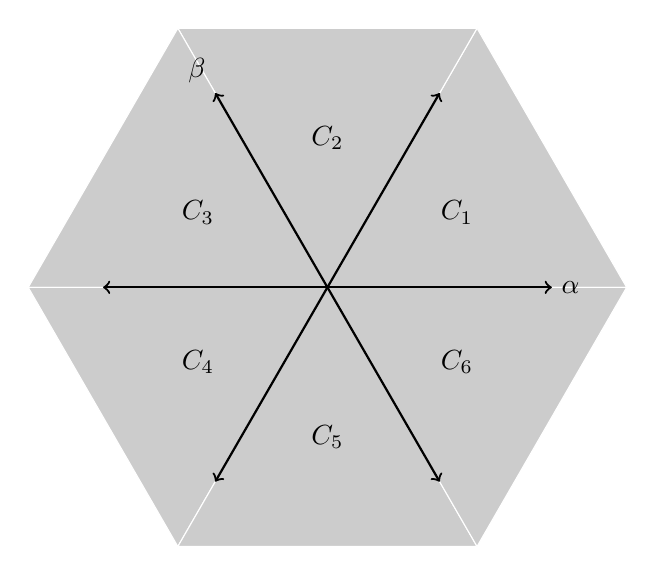
\begin{tikzpicture}[
    scale=0.95
    % arrow heads for all lines (with narrower arrow head width)
    %-{Straight Barb[bend,
       %width=\the\dimexpr10\pgflinewidth\relax,
       %length=\the\dimexpr12\pgflinewidth\relax]},
  ]
    %coordinate system
    %\draw[black] (-6,0) -- (6,0);
    %\draw[black] (0,-6) -- (0,6);
    % straight arrows
    \foreach \i in {0, 1, ..., 5} {
      \filldraw[fill=gray!40!white, draw=white] (0,0) -- (\i*60:4) -- (\i*60+60:4) -- (0,0) ;
    }
    \foreach \i in {0, 1, ..., 5} {
      \draw[->,thick, black] (0, 0) -- (\i*60:3);
    }
    % annotations
    \node[right] at (3, 0) {$\alpha$};
    %\node[above] at (1*60:3) {$\alpha + \beta$};
    \node[above left] at (2*60:3) {$\beta$};
    %\node[left] at (-3, 0) {$-\alpha$};
    %\node[below] at (4*60:3) {$-\alpha - \beta$};
    %\node[below] at (5*60:3) {$- \beta$};
    \foreach \i in {1, 2, ..., 6} {
      \node at (-30+\i*60:2) {$\mathfrak{C}_\i$};
    }
  \end{tikzpicture}
  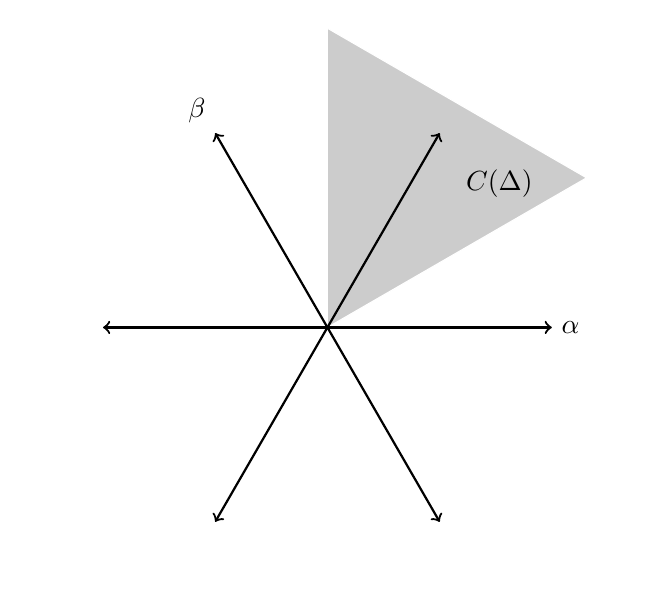
\begin{tikzpicture}[
      scale=0.95
    % arrow heads for all lines (with narrower arrow head width)
    %-{Straight Barb[bend,
       %width=\the\dimexpr10\pgflinewidth\relax,
       %length=\the\dimexpr12\pgflinewidth\relax]},
  ]
    %coordinate system
    %\draw[black] (-6,0) -- (6,0);
    %\draw[black] (0,-6) -- (0,6);
    % straight arrows
    \foreach \i in {0, 1, ..., 5} {
      \filldraw[fill=gray!00!white, draw=white] (0,0) -- (\i*60:4) -- (\i*60+60:4) -- (0,0) ;
    }
    \filldraw[fill=gray!40!white, draw=white] (0,0) -- (30:4) -- (90:4) -- (0,0) ;
    \foreach \i in {0, 1, ..., 5} {
      \draw[->,thick, black] (0, 0) -- (\i*60:3);
    }
    % annotations
    \node[right] at (3, 0) {$\alpha$};
    %\node[above] at (1*60:3) {$\alpha + \beta$};
    \node[above left] at (2*60:3) {$\beta$};
    %\node[left] at (-3, 0) {$-\alpha$};
    %\node[below] at (4*60:3) {$-\alpha - \beta$};
    %\node[below] at (5*60:3) {$- \beta$};
    \node at (40:3) {$\mathfrak{C}(\Delta)$};
  \end{tikzpicture}
  \caption{Das Wurzelsystem $\mathbf{A_2}$ mit den \weyl\hyp{}Kammern $\mathfrak{C}_1,\dots,\mathfrak{C}_6$ im linken Teil und mit der Fundamentalkammer $\mathfrak{C}(\Delta)$ zu $\Delta := \{\alpha, \beta\}$ im rechten Teil.}
\end{figure}


Dass $\Delta(\gamma)$ sogar ein Fundamentalsystem von $\Phi$ ist, lässt sich in \cite[S.48]{humphreys1972introduction} nachlesen.
Es gilt nämlich der folgende Satz.

\begin{thm}
  \label{thm:base}
  Sei $\Phi$ ein Wurzelsystem und $\gamma \in E$ diesbezüglich regulär.
  Dann ist die Menge $\Delta(\gamma)$ aller unzerlegbaren Wurzeln aus $\Phi^+(\gamma)$ ein Fundamentalsystem von $\Phi$ und jedes Fundamentalsystem ist von dieser Form. \qed
\end{thm}

\begin{defn}
  Sei $\Phi$ ein Wurzelsystem über $E$ mit Fundamentalsystem $\Delta$.
  Gilt $\Delta = \Delta(\gamma)$ für ein reguläres $\gamma \in E$, so bezeichnet man $\mathfrak{C}(\Delta) := \mathfrak{C}(\gamma)$ als \emph{Fundamentalkammer bezüglich} $\Delta$.
\end{defn}

Wir betrachten nun einen Spezialfall von Spiegelungsgruppen. Allgemeine Spiegelungsgruppen werden in \cite{humphreys1992reflection} behandelt.

\begin{defn}
  \label{def:weylgroup}
  Sei $\Phi$ ein Wurzelsystem über $E$. 
  Dann bezeichnet $\W$ die von den Spiegelungen $\sigma_\alpha$, $\alpha \in \Phi$, erzeugte Untergruppe der allgemeinen linearen Gruppe $\GL(E)$. 
  Man nennt $\W$ die \emph{\weyl\hyp{}Gruppe} von $\Phi$.
\end{defn}

Es lassen sich nun unterschiedliche von $\W$ induzierte Gruppenoperationen betrachten. Über deren Wohldefiniertheit gibt die nachfolgende Proposition Auskunft. 

Für den Beweis benötigen wir ein Lemma, welches das Verhalten von Spiegelungen aus der \weyl\hyp{}Gruppe unter Konjugation mit Vektorraumautomorphismen beschreibt. 
Der Beweis einer Verallgemeinerung dieses Lemmas findet sich in \cite[S.43]{humphreys1972introduction}.

\begin{lem}
  \label{lem:conjReflection}
  Sei $\Phi$ ein Wurzelsystem über $E$ mit \weyl\hyp{}Gruppe $\W$.
  Dann gilt 
  \begin{displaymath}
    \sigma \sigma_\alpha \sigma^{-1} = \sigma_{\sigma(\alpha)} 
  \end{displaymath}
  für alle $\sigma \in \W$ und alle $\alpha \in \Phi$. \qed
\end{lem}

\begin{prop}
  \label{prop:groupOp}
  Sei $\Phi$ ein Wurzelsystem über $E$ mit \weyl\hyp{}Gruppe $\W$.
  Dann gelten für alle $\gamma, \gamma' \in E$ und $\sigma \in \W$ die folgenden Aussagen:
  \begin{enumerate}[(a)]
    \item Es operiert $\W$ auf der Menge der regulären Elemente: 
      \begin{addmargin}[2em]{2em}
        Es ist $\sigma(\gamma)$ genau dann regulär, wenn $\gamma$ regulär ist.
      \end{addmargin}
      
    \item Aus $\mathfrak{C}(\gamma) = \mathfrak{C}(\gamma')$ folgt, dass auch $\mathfrak{C}(\sigma(\gamma)) = \mathfrak{C}(\sigma(\gamma'))$. \\
      Es operiert $\W$ auf der Menge der \weyl\hyp{}Kammern $\{\mathfrak{C}(\gamma) \mid \gamma \text{ regulär}\}$. Die Gruppeoperation lässt sich durch $ \sigma(\mathfrak{C}(\gamma)) = \mathfrak{C}(\sigma(\gamma))$ definieren.

    \item Es operiert $\W$ auf der Menge der Fundamentalsysteme $\{\Delta(\gamma) \mid \gamma \text{ regulär}\}$: 
      \begin{addmargin}[2em]{2em}
        Ist $\Delta$ ein Fundamentalsystem für $\Phi$, so auch $\sigma(\Delta)$. 
      \end{addmargin}

    \item Die unter (b) und (c) beschriebenen Gruppenoperationen sind kompatibel in dem Sinne, dass 
      $\sigma(\Delta(\gamma)) = \Delta(\sigma(\gamma))$
      und damit auch
      $\sigma(\mathfrak{C}(\Delta)) = \mathfrak{C}(\sigma(\Delta))$
      gilt.
  \end{enumerate}
\end{prop}

\begin{proof}
  (a): 
  Angenommen, $\sigma(\gamma)$ sei nicht regulär, dann existiert ein $\alpha \in \Phi$ mit $\sigma(\gamma) \in P_\alpha$.
  Damit folgt $\sigma(\gamma) = \sigma_\alpha \sigma(\gamma)$, da $\sigma_\alpha$ Elemente aus $P_\alpha$ fixiert.
  Hieraus ergibt sich mit Lemma \ref{lem:conjReflection} nun $\gamma = \sigma^{-1} \sigma_\alpha \sigma(\gamma) = \sigma_{\sigma(\alpha)}(\gamma)$, was wiederum $\gamma \in P_{\sigma(\alpha)}$ impliziert.
  Nach \hyperref[it:R3]{(R3)} gilt $\sigma(\alpha) \in \Phi$, also ist $\gamma$ im Widerspruch zur Voraussetzung nicht regulär.
  Die Annahme, dass $\sigma(\gamma)$ nicht regulär sei, muss also verworfen werden.
  
  Die Umkehrung der Aussage folgt aus der gezeigten Implikationsrichtung durch Anwendung der Spiegelung $\sigma^{-1}$ auf $\sigma(\gamma)$.

  (b): 
  Seien $\gamma, \gamma'$ regulär mit $\mathfrak{C}(\gamma) = \mathfrak{C}(\gamma')$.
  Angenommen, es sei $\mathfrak{C}(\sigma(\gamma)) \neq \mathfrak{C}(\sigma(\gamma'))$.
  Dann existiert ein $\alpha \in \Phi$, sodass einerseits $(\sigma(\gamma), \alpha) > 0$ und andererseits $(\sigma(\gamma'), \alpha) < 0$ gelten.
  Wir betrachten nun die Abbildung $x \mapsto  (\sigma(x), \alpha)$.
  Diese ist als Linearform auf dem endlichdimensionalen Vektorraum $E$ stetig bezüglich \euklid ischer Topologie.

  Da $\mathfrak{C}(\gamma)$ eine zusammenhängende Menge ist, folgt mit dem Zwischenwertsatz \cite[S.232]{bartsch2015allgemeine}, dass ein reguläres $x \in \mathfrak{C}(\gamma)$ existiert mit $(\sigma(x), \alpha) = 0$.
  Das bedeutet jedoch gerade, dass $\sigma(x)$ ein Element von $P_\alpha$ ist und damit wäre $\sigma(x)$ nicht regulär.
  Dies steht jedoch im Widerspruch zu (a). 
  Es muss also auch $\mathfrak{C}(\sigma(\gamma)) = \mathfrak{C}(\sigma(\gamma'))$ gelten.
  
  Sei nun für den zweiten Teil der zu beweisenden Aussage $x \in \mathfrak{C}(\sigma(\gamma))$.
  Daraus folgt $\mathfrak{C}(x) = \mathfrak{C}(\sigma(\gamma))$.
  Dann gilt nach der soeben bewiesenen Aussage auch $\mathfrak{C}(\sigma^{-1}(x)) = \mathfrak{C}(\gamma)$.
  Insbesondere gilt also $\sigma^{-1}(x) \in \mathfrak{C}(\gamma)$ und damit auch $x \in \sigma(\mathfrak{C}(\gamma))$
  
  Die umgekehrte Inklusion folgt analog: Ist $x \in \sigma(\mathfrak{C}(\gamma))$, so ist $\sigma(x) \in \mathfrak{C}(\gamma)$ und damit gilt $\mathfrak{C}(\sigma(x)) = \mathfrak{C}(\gamma)$. 
  Wie schon gezeigt, folgt aus der Betrachtung von Bildern unter $\sigma^{-1} = \sigma$ sofort $\mathfrak{C}(x) = \mathfrak{C}(\sigma(\gamma))$, also insbesondere $x \in \mathfrak{C}(\sigma(\gamma))$.

  (c): 
  Da $\sigma$ als orthogonale Abbildung insbesondere injektiv ist, folgt, dass $\sigma(\Delta)$ wieder ein System linear unabhängiger Vektoren und damit aufgrund von \hyperref[it:B1]{(B1)} wieder eine Vektorraumbasis von $E$ ist.
  
  Ist nun $\beta \in \Phi$ mit der nach \hyperref[it:B2]{(B2)} existierenden Darstellung $\beta = \sum_{\alpha \in \Delta} k_\alpha \alpha$ gegeben, so gilt
  \begin{displaymath}
  \sigma(\beta) 
    = \sigma(\sum_{\alpha \in \Delta} k_\alpha \alpha)
    = \sum_{\alpha \in \Delta} k_\alpha \sigma(\alpha)
    = \sum_{\sigma(\alpha) \in \sigma(\Delta)} k_\alpha \sigma(\alpha)
  \end{displaymath}
  aufgrund der Linearität von $\sigma$.
  Die Vorzeichen der Linearfaktoren $k_\alpha$ bleiben zudem unverändert, womit \hyperref[it:B2]{(B2)} folgt.
  Damit ist auch $\sigma(\Delta)$ ein Fundamentalsystem.

  (d):
  Wir stellen zunächst fest, dass aufgrund der Aussage (c), die zu zeigende Gleichheit in dem Sinne wohldefiniert ist, dass $\sigma(\Delta(\gamma))$ als Bild eines Fundamentalsystems wieder ein Fundamentalsystem darstellt.

  Sei nun $\sigma(\alpha) \in \sigma(\Delta(\gamma))$.
  Mit $\alpha \in \Delta(\gamma)$ gilt definitionsgemäß $(\alpha, \gamma) > 0$.
  Spiegelungen erhalten als Isometrien das Skalarprodukt, es gilt also auch $(\sigma(\alpha), \sigma(\gamma)) > 0$.
  Dies wiederum impliziert $\sigma(\alpha) \in \Phi^+(\sigma(\gamma))$.
  Angenommen, $\sigma(\alpha)$ wäre eine zerlegbare Wurzel.
  Dann ist auch $\alpha$ zerlegbar, da $\sigma$ bijektiv ist.
  Dies steht jedoch im Widerspruch dazu, dass mit $\alpha \in \Delta$ die Wurzel $\alpha$ als einfach vorausgesetzt wurde.
  Also muss $\sigma(\alpha)$ auch einfach sein, womit $\sigma(\alpha) \in \Delta(\sigma(\gamma))$ folgt.
  Das impliziert die Gültigkeit der Inklusion $\sigma(\Delta(\gamma)) \subseteq \Delta(\sigma(\gamma))$.
  
  Da $\sigma$ bijektiv ist und beide Mengen als Teilmengen des endlichen Wurzelsystems $\Phi$ auch endlich sind, folgt hiermit bereits die Gleichheit.
\end{proof}

Mit weiteren Eigenschaften dieser Gruppenoperationen werden wir uns in Abschnitt \ref{sec:weylgroup} beschäftigen.
